\chapter{Anforderungen und Systemkonzept}
\label{chap:anforderungen}

Dieses Kapitel definiert die technischen Spezifikationen und beschreibt das übergeordnete Systemkonzept des Motorcontrollers. Aus den Randbedingungen des Antriebsstrangs werden die elektrischen Anforderungen abgeleitet, welche die Grundlage für die spätere Komponentenauswahl und die thermische Dimensionierung bilden. Anschließend wird die gewählte Systemarchitektur sowie das softwareseitige Ansteuerverfahren begründet.

% ============================================================
\section{Elektrische Anforderungen}
\label{sec:anforderungen_elektrisch}

Das Antriebssystem basiert auf zwei bürstenlosen Gleichstrommotoren mit einer Nennleistung von jeweils $400\,\mathrm{W}$. Die elektrische Energieversorgung erfolgt über einen Lithium-Ionen-Akkumulator mit einer Nominalspannung von $36\,\mathrm{V}$ und einer Kapazität von $4{,}4\,\mathrm{Ah}$. Aus diesen Randbedingungen ergeben sich spezifische Anforderungen an die Spannungsfestigkeit, Stromtragfähigkeit sowie die dynamischen Eigenschaften der eingesetzten Leistungselektronik.

Die Auslegung der Betriebsspannung orientiert sich an der Charakteristik des verwendeten Akkus. Bei dem eingesetzten Energiespeicher handelt es sich um ein in Serie verschaltetes 10S-Lithium-Ionen-Pack, dessen maximale Ladeschlussspannung etwa $42\,\mathrm{V}$ beträgt. Während des Betriebs eines Traktionsantriebs können zusätzlich kurzzeitige transiente Überspannungen auftreten. Diese entstehen insbesondere durch parasitäre Leitungsinduktivitäten in Kombination mit den schnellen Schaltvorgängen der Leistungshalbleiter. Ein weiterer relevanter Effekt ist ein möglicher Spannungsanstieg im Zwischenkreis während generatorischer Betriebszustände, beispielsweise beim rekuperativen Bremsen. Um einen zuverlässigen und sicheren Betrieb zu gewährleisten, müssen alle leistungstragenden Komponenten des Inverters, insbesondere die MOSFETs und die Zwischenkreiskondensatoren, daher für eine Spannungsfestigkeit von mindestens $60\,\mathrm{V}$ ausgelegt werden. In der Praxis wird aus Gründen der Bauteilzuverlässigkeit und zur Berücksichtigung zusätzlicher Sicherheitsreserven häufig eine Spannungsfestigkeit von bis zu $80\,\mathrm{V}$ gewählt.

Neben der Spannungsfestigkeit stellt die Stromtragfähigkeit der Endstufe eine zentrale Entwurfsgröße dar. Bei einer mechanischen Nennleistung von $400\,\mathrm{W}$ und einer elektrischen Nennspannung von $36\,\mathrm{V}$ ergibt sich im stationären Nennbetrieb ein Strom von etwa $11{,}1\,\mathrm{A}$ pro Motor. Für die thermische Auslegung der Leistungselektronik ist jedoch nicht ausschließlich dieser stationäre Betriebszustand maßgeblich. Insbesondere während dynamischer Betriebsphasen, etwa beim Beschleunigen aus dem Stillstand, treten deutlich höhere Stromwerte auf. In diesem Arbeitspunkt ist die induzierte Gegenspannung des Motors noch gering beziehungsweise im Stillstand vollständig null. Der Strom wird folglich im Wesentlichen durch den ohmschen Widerstand der Motorwicklungen sowie durch parasitäre Serienwiderstände der Stromversorgung begrenzt. Daraus resultieren kurzzeitige Stromspitzen, die typischerweise ein Mehrfaches des Nennstroms erreichen können.

Um diesen transienten Belastungen Rechnung zu tragen und eine ausreichende thermische Robustheit der Endstufe sicherzustellen, wird die Leistungselektronik für einen kontinuierlich zulässigen Phasenstrom von etwa $30\,\mathrm{A}$ (RMS) dimensioniert. Hierbei entspricht dieser Effektivwert einem periodischen Spitzenstrom von $\hat{i} = \sqrt{2} \cdot 30\,\mathrm{A} \approx 42{,}4\,\mathrm{A}$. Dieser Spitzenwert ist die kritische Auslegungsgröße für die Safe Operating Area (SOA) der Transistoren und für die Auslegung der Gate-Treiber. Diese Auslegung berücksichtigt sowohl kurzzeitige Anlaufströme als auch mögliche Betriebszustände mit erhöhter Last. Gleichzeitig definiert diese Stromanforderung die Randbedingungen für die Dimensionierung der Leiterplattenkupferflächen, der Leiterquerschnitte sowie der Kühlstruktur der eingesetzten Leistungshalbleiter. Darüber hinaus beeinflusst der maximal zulässige Strom direkt die Auswahl geeigneter MOSFETs, insbesondere im Hinblick auf einen möglichst geringen Einschaltwiderstand $R_{\mathrm{DS(on)}}$, um die leitungsbedingten Verluste und damit die thermische Belastung zu minimieren.

Im Zusammenhang mit der Stromdimensionierung ist zwischen dem Phasenstrom der Motorwicklungen und dem vom Energiespeicher gelieferten Gleichstrom zu unterscheiden. Durch das Pulsweitenmodulationsverfahren verhält sich der dreiphasige Inverter funktional ähnlich zu einem leistungselektronischen Abwärtswandler. Bei einer sinusförmigen Strangstromform lässt sich der aufgenommene Gleichstrom über den Modulationsindex $m$ und den Leistungsfaktor $\cos(\varphi)$ näherungsweise beschreiben mit $I_{\mathrm{DC}} \approx \frac{3}{2} \cdot m \cdot I_{\mathrm{phase, max}} \cdot \cos(\varphi)$ \cite{Mohan2003}. Insbesondere bei niedrigen Drehzahlen (kleiner Modulationsindex $m$) kann folglich ein relativ hoher Phasenstrom im Motor fließen, während der vom Energiespeicher entnommene Gleichstrom deutlich geringer bleibt. Für die Auslegung der Leistungselektronik ist daher der lokal im Inverter auftretende Phasenstrom die maßgebliche Größe, während der dauerhaft verfügbare Systemstrom durch das Battery-Management-System (BMS) des Akkumulators begrenzt wird.

Ein weiterer relevanter Entwurfsparameter ist die gewählte Pulsweitenmodulationsfrequenz. Zur Vermeidung wahrnehmbarer akustischer Emissionen des Motors sowie zur Reduktion des Stromrippels wird eine Schaltfrequenz oberhalb der menschlichen Hörschwelle angestrebt. In dieser Arbeit wird daher eine PWM-Frequenz von $f_{\mathrm{SW}} = 20\,\mathrm{kHz}$ angenommen. Diese Frequenz stellt einen technischen Kompromiss dar \cite{Erickson2020}. Da sich die Stromwelligkeit $\Delta I$ umgekehrt proportional zur Schaltfrequenz verhält ($\Delta I \approx \frac{V_{\mathrm{DC}} \cdot D}{L \cdot f_{\mathrm{SW}}}$), wird mit steigender Schaltfrequenz eine glattere Stromform erreicht. Gleichzeitig steigen jedoch die Schaltverluste der Leistungshalbleiter sowie die Anforderungen an die Gate-Treiber an. Die gewählte Frequenz ermöglicht somit eine ausreichend glatte Stromform bei gleichzeitig moderaten Schaltverlusten und stellt einen geeigneten Betriebsbereich für kompakte Traktionsantriebe dieser Leistungsklasse dar.


Zur besseren Übersicht sind die abgeleiteten elektrischen Anforderungen für den nachfolgenden Hardware-Entwurf in Tabelle \ref{tab:anforderungen} zusammengefasst.

\begin{table}[htbp]
\centering
\caption{Zusammenfassung der elektrischen Systemanforderungen.}
\label{tab:anforderungen}
\begin{tabular}{llll}
\toprule
\textbf{Parameter} & \textbf{Symbol} & \textbf{Wert} & \textbf{Einheit} \\
\midrule
Nennspannung des Akkumulators & $V_{\mathrm{bat,nom}}$ & 36 & V \\
Maximale Akkumulatorspannung & $V_{\mathrm{bat,max}}$ & 42 & V \\
MOSFET-Spannungsfestigkeit & $V_{\mathrm{DS,max}}$ & $\ge 60$ & V \\
Elektrische Nennleistung & $P_{\mathrm{nom}}$ & 400 & W \\
Maximaler Phasenstrom & $I_{\mathrm{phase,max}}$ & 30 & A$_{\mathrm{RMS}}$ \\
PWM-Schaltfrequenz & $f_{\mathrm{SW}}$ & 20 & kHz \\
Logikpegel des Mikrocontrollers & $V_{\mathrm{logic}}$ & 3.3 & V \\
\bottomrule
\end{tabular}
\end{table}

% ============================================================
\section{Systemarchitektur}
\label{sec:systemarchitektur}

Um die abgeleiteten Anforderungen umzusetzen, wird der Motorcontroller in eine modulare Hardwarearchitektur gegliedert. Das Gesamtsystem besteht aus drei funktionalen Hauptblöcke. Der digitalen Steuerungseinheit, der analogen Treiberstufe und dem Leistungsteil. Abbildung \ref{fig:blockschaltbild} zeigt das Blockdiagramm des Motorcontrollers.

\begin{figure}[htbp]
    \centering
    \resizebox{\textwidth}{!}{
    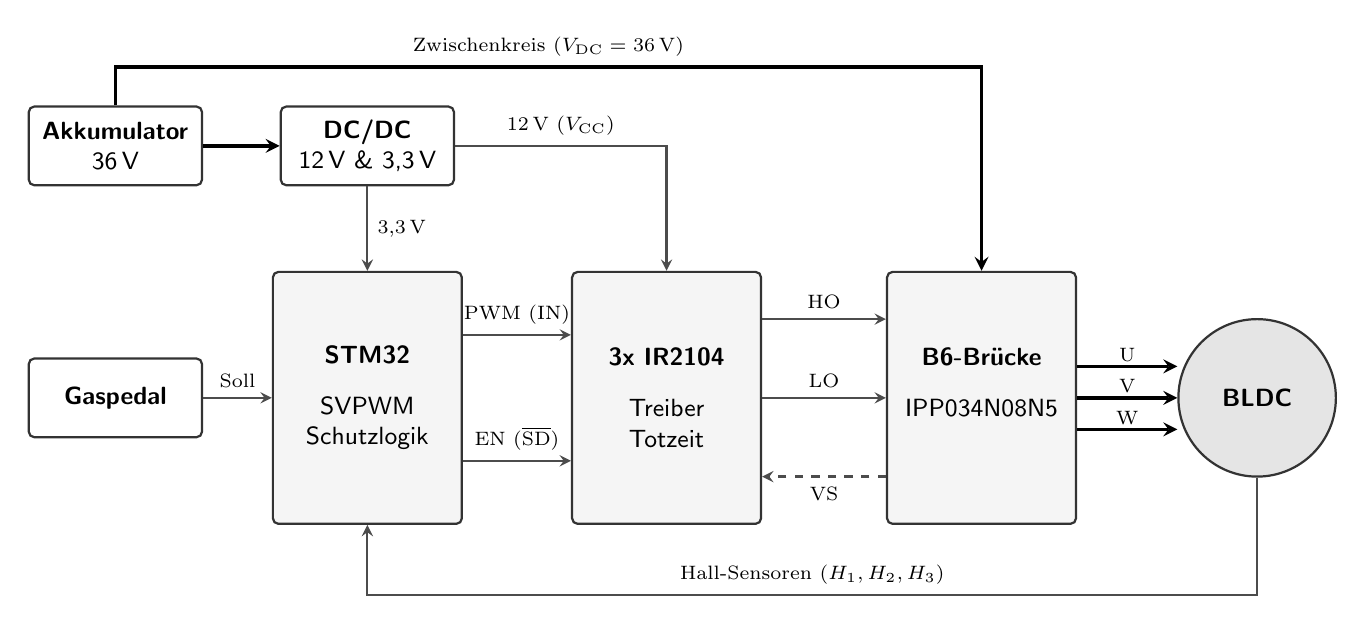
\begin{tikzpicture}[
        >=stealth,
        font=\sffamily\small,
        % Kompaktere Block-Stile
        mainblock/.style={draw=black!80, fill=black!4, thick, rectangle, minimum height=3.2cm, minimum width=2.4cm, align=center, rounded corners=2pt},
        smallblock/.style={draw=black!80, fill=white, thick, rectangle, minimum height=1.0cm, minimum width=2.2cm, align=center, rounded corners=2pt},
        motorblock/.style={draw=black!80, fill=black!10, thick, circle, minimum size=2.0cm, align=center},
        signal/.style={->, thick, draw=black!70},
        power/.style={->, very thick, draw=black}
    ]

    % ==========================================
    % 1. KNOTEN (BLÖCKE) PLATZIEREN
    % ==========================================
    
    % Eingänge (Links)
    \node[smallblock] (throttle) at (0, 0) {\textbf{Gaspedal}};
    \node[smallblock] (battery)  at (0, 3.2) {\textbf{Akkumulator} \\ 36\,V};
    
    % DC/DC Versorgung
    \node[smallblock] (dcdc) at (3.2, 3.2) {\textbf{DC/DC} \\ 12\,V \& 3,3\,V};

    % Hauptblöcke (Mitte bis Rechts)
    \node[mainblock] (mcu) at (3.2, 0) {\textbf{STM32} \\[0.8em] SVPWM \\ Schutzlogik};
    
    \node[mainblock] (driver) at (7.0, 0) {\textbf{3x IR2104} \\[0.8em] Treiber \\ Totzeit};
    
    \node[mainblock] (inverter) at (11.0, 0) {\textbf{B6-Brücke} \\[0.8em] IPP034N08N5 \\};

    % Aktor (Ganz rechts)
    \node[motorblock] (motor) at (14.5, 0) {\textbf{BLDC}};


    % ==========================================
    % 2. VERBINDUNGEN ZIEHEN
    % ==========================================

    % --- Leistungs- und Versorgungsleitungen ---
    \draw[power] (battery.east) -- (dcdc.west);
    
    % 36V Leitung (oben)
    \draw[power] (battery.north) |- (0, 4.2) -| (inverter.north) node[pos=0.25, above, font=\scriptsize] {Zwischenkreis ($V_{\mathrm{DC}} = 36\,\mathrm{V}$)};
    
    % Phasen zum Motor
    \draw[power] ([yshift=0.4cm]inverter.east) -- ([yshift=0.4cm]motor.west) node[midway, above, yshift=-2pt, font=\scriptsize] {U};
    \draw[power] ([yshift=0cm]inverter.east) -- ([yshift=0cm]motor.west) node[midway, above, yshift=-2pt, font=\scriptsize] {V};
    \draw[power] ([yshift=-0.4cm]inverter.east) -- ([yshift=-0.4cm]motor.west) node[midway, above, yshift=-2pt, font=\scriptsize] {W};

    % --- Signalleitungen ---
    \draw[signal] (dcdc.south) -- (mcu.north) node[midway, right, font=\scriptsize] {3,3\,V};
    \draw[signal] (dcdc.east) -| (driver.north) node[near start, above, font=\scriptsize] {12\,V ($V_{\mathrm{CC}}$)};

    \draw[signal] (throttle.east) -- (mcu.west) node[midway, above, font=\scriptsize] {Soll};

    % MCU zu Driver
    \draw[signal] ([yshift=0.8cm]mcu.east) -- ([yshift=0.8cm]driver.west) node[midway, above, font=\scriptsize] {PWM (IN)};
    \draw[signal] ([yshift=-0.8cm]mcu.east) -- ([yshift=-0.8cm]driver.west) node[midway, above, font=\scriptsize] {EN ($\overline{\mathrm{SD}}$)};

    % Driver zu Inverter
    \draw[signal] ([yshift=1.0cm]driver.east) -- ([yshift=1.0cm]inverter.west) node[midway, above, font=\scriptsize] {HO};
    \draw[signal] ([yshift=0cm]driver.east) -- ([yshift=0cm]inverter.west) node[midway, above, font=\scriptsize] {LO};
    \draw[signal, dashed] ([yshift=-1.0cm]inverter.west) -- ([yshift=-1.0cm]driver.east) node[midway, below, font=\scriptsize] {VS};

    % --- Feedback ---
    \draw[signal] (motor.south) |- (14.5, -2.5) -| (mcu.south) node[pos=0.25, above, font=\scriptsize] {Hall-Sensoren ($H_1, H_2, H_3$)};

    \end{tikzpicture}
    }
    \caption{Systemarchitektur des Motorcontrollers.}
    \label{fig:blockschaltbild}
\end{figure}

Die Steuerungsebene wird durch einen STM32-Mikrocontroller abgebildet, welcher mit einem Logikpegel von $3{,}3\,\mathrm{V}$ arbeitet. Dieser erfasst die Signale der Hall-Sensoren und generiert die hochfrequenten PWM-Signale. Da die Leistungshalbleiter (N-Kanal-MOSFETs) eine Gate-Source-Spannung von typischerweise $10\,\mathrm{V}$ bis $15\,\mathrm{V}$ benötigen, um vollständig und verlustarm durchzusteuern, fungiert der Halbbrückentreiber IR2104 als Pegelwandler und Leistungsverstärker. Er bildet die Schnittstelle zwischen der empfindlichen $3{,}3\,\mathrm{V}$-Logik und der Leistungsebene. Die Leistungsebene selbst besteht aus der dreiphasigen B6-Wechselrichterbrücke sowie dem Gleichspannungszwischenkreis. Letzterer wird durch Elektrolytkondensatoren realisiert und erfüllt eine entscheidende Pufferfunktion. Er stellt die hochfrequenten, pulsförmigen Rippleströme des Inverters lokal zur Verfügung und minimiert so transiente Spannungseinbrüche auf der Batteriezuleitung.

% ============================================================
\section{Gewähltes Ansteuerverfahren}
\label{sec:ansteuerverfahren}

Die Wahl des Ansteuerverfahrens beeinflusst sowohl die Komplexität der Softwarearchitektur als auch die Rechenlast des eingesetzten Mikrocontrollers. Für den im Rahmen dieser Arbeit entwickelten Prototypen wurde daher ein bewusst reduzierter Ansatz gewählt.

Der Antrieb wird im Open-Loop-Betrieb betrieben, sodass auf eine geschlossene Drehmoment- oder Drehzahlregelung verzichtet wird. Insbesondere wird keine feldorientierte Regelung implementiert. Eine FOC erfordert neben einer präzisen Rotorlagebestimmung zusätzliche zeitkritische Strommessungen in mindestens zwei Motorphasen. Darüber hinaus sind mehrere mathematische Transformationen, insbesondere die Clarke- und Park-Transformation, notwendig, wodurch die algorithmische Komplexität sowie die Anforderungen an die Echtzeitfähigkeit des Mikrocontrollers erheblich steigen. Da der Schwerpunkt dieser Arbeit auf der Entwicklung und Auslegung der leistungselektronischen Hardware sowie auf der thermischen Beherrschung der Endstufe liegt, wird auf eine Implementierung verzichtet.

Zur Modulation der dreiphasigen Ausgangsspannungen wird jedoch nicht auf eine einfache Blockkommutierung zurückgegriffen. Stattdessen wird eine SVPWM eingesetzt. Die grundlegende Rotorlageinformation wird dabei aus den vorhandenen Hall-Sensorsignalen gewonnen. Da diese Sensoren systembedingt nur eine diskrete Winkelauflösung von $60^\circ$ elektrisch liefern, wird die exakte Rotorposition zwischen zwei Schaltflanken durch den Mikrocontroller geschätzt. Dies erfolgt über eine lineare Winkelinterpolation, welche auf der hochauflösenden Zeitmessung der vorangegangenen Durchlaufzeit basiert. Wie in Abschnitt \ref{sec:modulation} gezeigt wird, ermöglicht die SVPWM eine etwa $15\,\%$ bessere Ausnutzung der verfügbaren Zwischenkreisspannung im Vergleich zu einer sinusförmigen Pulsweitenmodulation. Dieser Vorteil ist im vorliegenden $36\,\mathrm{V}$-System besonders relevant, da die maximal erreichbare Motordrehzahl und damit die mögliche Fahrzeuggeschwindigkeit unmittelbar von der nutzbaren Zwischenkreisspannung abhängen.